\documentclass[12pt]{article} % Clase de documento: artículo y tamaño de letra
\usepackage[utf8]{inputenc} % Escritura en castellano con acentos
\usepackage[T1]{fontenc} % Escritura en castellano con acentos
\usepackage{calligra} 
\usepackage{pslatex}  % Fuente de letras
\usepackage{graphicx}
\usepackage[margin=2.5cm]{geometry}
\usepackage{txfonts}
\usepackage{xcolor}
\usepackage{fancyhdr}
\usepackage{graphicx}
\usepackage{float}
\usepackage{listings}
\usepackage{multicol}
\usepackage{color}
\usepackage{times}
\usepackage{tikz}
\usepackage{verbatim}
\usepackage{mdwlist}
\usepackage{array}
\usepackage{caption}

\usetikzlibrary{chains,fit,shapes,arrows,calc,shapes,decorations.pathreplacing}


\pagestyle{fancy}
\headheight=50pt %para cambiar el tamaño del encabezado
\fancyhead[L]    %la "L" indica a la izquierda
{	
 \begin{minipage}{3.3cm}
  
\includegraphics[width=1.0\textwidth]{Logo-UTN-BA.jpeg}
%  
\includegraphics[width=0.6\textwidth]{UTNlogo.eps}
 \end{minipage}	
 \begin{minipage}{7.7cm}
   \normalsize
   {
     \textsf
     {
       \calligra{Universidad Tecnológica Nacional\\ Facultad Regional Buenos Aires \\ Departamento de {Ingeniería} {Electrónica}} 
     }
   }
 \end{minipage}
}

\fancyhead[R] %la "R" indica a la derecha
{
  \begin{minipage}{4.0cm}
   \small
   {
     \emph{\textbf{Informática I}} \\ \emph{\today} \\ \emph{Ejercitación con punteros}\\ \emph{Curso r1092}  
   }
  \end{minipage}}


\begin{document} % Inicio del documento
% \renewcommand{\baselinestretch}{1.5}
\newpage
%Cambia de página, el texto después de este comando aparecerá en la siguiente página en adelante.

Dada la declaración de las siguientes variables y su representación en memoria \\
int	a , b , *p , *q , **r , **s;\\
Complete la siguiente tabla con los valores que tomarán las variables y lo apuntado por sus contenidos en las columnas correspondientes.\\
Cuando no sea posible indicar un valor, señalelo con el signo  -?-  \\
Las letras $\alpha$ , $\beta$ , $\chi$ ,$\delta$ ,$\epsilon$ y $\phi$ simbolizan las direcciones de memoria en las que se encuentran ubicadas las variables.\\ 
%\vspace{0.6cm}
\noindent

\lstset{
	frame=Ltb,
	framerule=0pt,
	aboveskip=0.5cm,
	framextopmargin=3pt,
	framexbottommargin=3pt,
	framexleftmargin=0.4cm,
	framesep=0pt,
	rulesep=.4pt,
	backgroundcolor=\color{gray97},
	rulesepcolor=\color{black},
% 	language=C,
	captionpos=b,
	tabsize=3,
	frame=lines,
	keywordstyle=\color{blue},
	commentstyle=\color{Gray},
	stringstyle=\color{red},
	numbers=left,
	numberstyle=\tiny,
	numbersep=5pt,
	breaklines=true,
	showstringspaces=false,
	basicstyle=\ttfamily\scriptsize,
	emph={label},
	framerule=0pt,
}

   \begin{center}
   \begin{tabular}{| c | c | c | c | c | c | c | c | c | c | c | c | c |}
    \hline
     expresión 					& a & b & p & q & *p & *q & r & s & *r & *s & **r & **s \\ \hline 
     a = 9 ; b = 4   			&   &   &   &   &    &    &   &   &    &    &     &     \\ \hline 
     p = \& a ; q = \& b  		&   &   &   &   &    &    &   &   &    &    &     &     \\ \hline 
     r= \& p ; s= \& q			&   &   &   &   &    &    &   &   &    &    &     &     \\ \hline 
     **r = *q  					&   &   &   &   &    &    &   &   &    &    &     &     \\ \hline 
     *p = *q + **s		   		&   &   &   &   &    &    &   &   &    &    &     &     \\ \hline 
     r = s ; q = p				&   &   &   &   &    &    &   &   &    &    &     &     \\ \hline 
     *( \& a ) = *( \& b )		&   &   &   &   &    &    &   &   &    &    &     &     \\ \hline 
     b = a - **r + *p			&   &   &   &   &    &    &   &   &    &    &     &     \\ \hline 
     *p = a	   					&   &   &   &   &    &    &   &   &    &    &     &     \\ \hline 
     q = \& b ; r = \& p		&   &   &   &   &    &    &   &   &    &    &     &     \\ \hline 
     *q = *q - **s + **( \& p )	&   &   &   &   &    &    &   &   &    &    &     &     \\ \hline 
   \end{tabular}	
  \end{center}
\noindent
 
\begin{center}
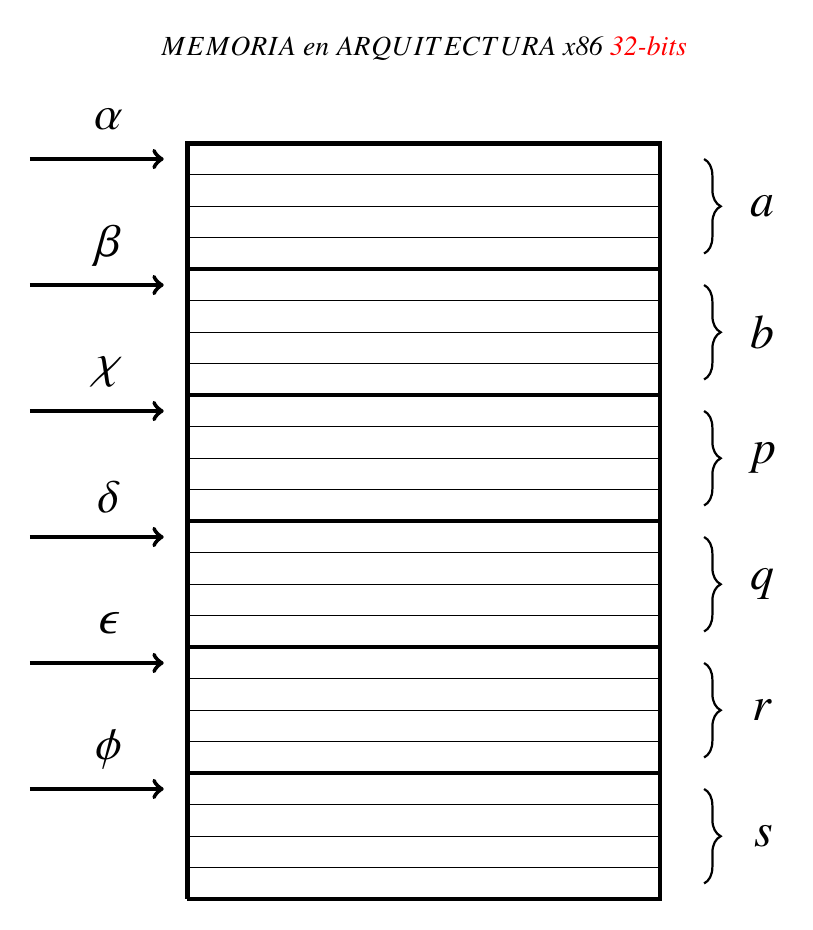
\begin{tikzpicture}
  \draw [ultra thick](-3,-6) -- (3,-6) -- (3,3.6) -- (-3,3.6) -- (-3,-6);
  \draw (-3,-5.6) -- (3,-5.6);
  \draw (-3,-5.2) -- (3,-5.2);
  \draw (-3,-4.8) -- (3,-4.8);
  \draw [ultra thick](-3,-4.4) -- (3,-4.4);
  \draw (-3,-4) -- (3,-4);
  \draw (-3,-3.6) -- (3,-3.6);
  \draw (-3,-3.2) -- (3,-3.2);
  \draw [ultra thick](-3,-2.8) -- (3,-2.8);
  \draw (-3,-2.4) -- (3,-2.4);
  \draw (-3,-2) -- (3,-2);
  \draw (-3,-1.6) -- (3,-1.6);
  \draw [ultra thick](-3,-1.2) -- (3,-1.2);
  \draw (-3,-0.8) -- (3,-0.8);
  \draw (-3,-0.4) -- (3,-0.4);
  \draw (-3,0) -- (3,0);
  \draw [ultra thick](-3,0.4) -- (3,0.4);
  \draw (-3,0.8) -- (3,0.8);
  \draw (-3,1.2) -- (3,1.2);
  \draw (-3,1.6) -- (3,1.6);
  \draw [ultra thick](-3,2) -- (3,2);
  \draw (-3,2.4) -- (3,2.4);
  \draw (-3,2.8) -- (3,2.8);
  \draw (-3,3.2) -- (3,3.2);

  \draw[	decorate,decoration={brace,raise=16pt,amplitude=6pt}, thick]
    (3,3.4) -- (3,2.2) node [black,midway,xshift=1.3cm]{\LARGE $a$};
  \draw[	decorate,decoration={brace,raise=16pt,amplitude=6pt}, thick]
    (3,1.8) -- (3,0.6) node [black,midway,xshift=1.3cm]{\LARGE $b$};
  \draw[	decorate,decoration={brace,raise=16pt,amplitude=6pt}, thick]
    (3,0.2) -- (3,-1) node [black,midway,xshift=1.3cm]{\LARGE $p$};
  \draw[	decorate,decoration={brace,raise=16pt,amplitude=6pt}, thick]
    (3,-1.4) -- (3,-2.6) node [black,midway,xshift=1.3cm]{\LARGE $q$};
  \draw[	decorate,decoration={brace,raise=16pt,amplitude=6pt}, thick]
    (3,-3) -- (3,-4.2) node [black,midway,xshift=1.3cm]{\LARGE $r$};
  \draw[	decorate,decoration={brace,raise=16pt,amplitude=6pt}, thick]
    (3,-4.6) -- (3,-5.8) node [black,midway,xshift=1.3cm]{\LARGE $s$};

  \draw[ultra thick,->] (-5,3.4) -- (-3.3,3.4);
  \draw[ultra thick,->] (-5,1.8) -- (-3.3,1.8);
  \draw[ultra thick,->] (-5,0.2) -- (-3.3,0.2);
  \draw[ultra thick,->] (-5,-1.4) -- (-3.3,-1.4);
  \draw[ultra thick,->] (-5,-3) -- (-3.3,-3);
  \draw[ultra thick,->] (-5,-4.6) -- (-3.3,-4.6);

  \node at (-4,3.9) {\LARGE $\alpha$};
  \node at (-4,2.3) {\LARGE $\beta$};
  \node at (-4,0.7) {\LARGE $\chi$};
  \node at (-4,-0.9) {\LARGE $\delta$};
  \node at (-4,-2.5) {\LARGE $\epsilon$};
  \node at (-4,-4.1) {\LARGE $\phi$};
  
  \node at (0,4.8) {\normalsize  \itshape $MEMORIA$ en $ARQUITECTURA$ x86 \textcolor{red}{32-bits}};
\end{tikzpicture}
\end{center}
 
\end{document} % Fin del documento.
